\subsection{Approach}
\label{sec:approach}

The introduction to this thesis stated its main objective, namely the
development of a deployable stand-alone model for precisely predicting tweet
engagement metrics.
As previously elaborated, `deployable' in this context stands for the practical
applicability of the model.
The term `stand-alone' denotes the requirement of solely relying
on data that stems directly from tweet objects of the public Twitter interface.
Not being dependent on additional data would enable the system to be applicable
in a streaming setting.
Furthermore, predicted engagement metrics should incorporate both eventual
retweet and favorite counts.
This section comprises three parts.
Firstly, limitations of the previously described prior work with regard to the
stated objective are outlined.
Secondly, the experiments conducted in this thesis are introduced.
Finally, necessary assumptions for the developed models are stated and justified.

\subsubsection{Limitations of prior research}

This thesis aims to develop deep learning models for predicting tweet
engagement.
Employing deep learning should help to overcome several limitations of prior
work in this research area (see ch.~\ref{sub:meth_prior_work}), which will be listed in the following.
Some of the described models rely on complex, manually crafted features, e.g.,
activity, topic similarity and relationship features.
These often require additional data and excessive preprocessing, in some cases
even precalculated models on separate data sets.
This stands in contrast to the ad-hoc processing requirement in the objective.
The hypothesis of this work is that these features can be omitted or
learned intrinsically by deep neural networks.
Manual feature creation is necessary for machine learning models like logistic
regression or decision trees that are less capable of creating own feature
representations.
Deep neural networks achieve higher representational capability by effectively
stacking non-linear modules which learn discrete features according to the problem at
hand~\footcite{LeCun2015}.
One objective for this thesis is an accurate prediction of the eventual popularity
of tweets.
Previous models mostly focus on probability prediction or binary classification
which is insufficient to meet this objective.
Furthermore, less complex models have not shown good performance in the multi-class
classification setting, only showing good accuracy for extreme cases.
This work tries to overcome this limitation by employing deep models on diverse
data sets with varying class distributions.
Following this approach should also conquer biases in the collected data.
In previous research, data sets were often collected around a single topic or
trend, sometimes even handpicked~\footcite{Zaman2014}.
Both models that apply predictive models in a regression setting are dependent
on some form of time-series observation of the retweet graph, which is not adequate for
an accurate prediction about future engagement at the time of tweet creation.
In this work, models are able to make real-time predictions, i.e., it could
be possible to deploy them in an application that is fed data from the Twitter
Streaming API~\footnote{\url{https://developer.twitter.com/en/docs/tweets/filter-realtime/overview/powertrack-api}}.
An additional feature of models in this work is their capability to predict both
number of retweets and favorites.

\subsubsection{Developed models}

Models developed in this thesis make use of content and contextual features,
inspired by previous work in this field.
Since the models only rely on tweet objects from the Twitter API, contextual
features are mainly limited to information about the source user~\footnote{\url{https://developer.twitter.com/en/docs/tweets/data-dictionary/overview/intro-to-tweet-json}}.
In contrast to previous model, sophisticated deep learning models should allow
more precise processing of tweet content, particularly because deep neural networks
show good performance on natural language processing tasks (see ch.~\ref{sub:dl_app_nlp}).
In summary, the deep models are fed both structured and unstructured data.
Here, structured data represents inputs that could easily be stored in
tabular format, e.g., a relational database.
Examples for these features include number of hashtags and URLs on the content
side, as well as follower count and account age on the contextual side.
The actual tweet content can be seen as unstructured data, due to its variation
in length and manifestation.

\begin{figure}[h]
  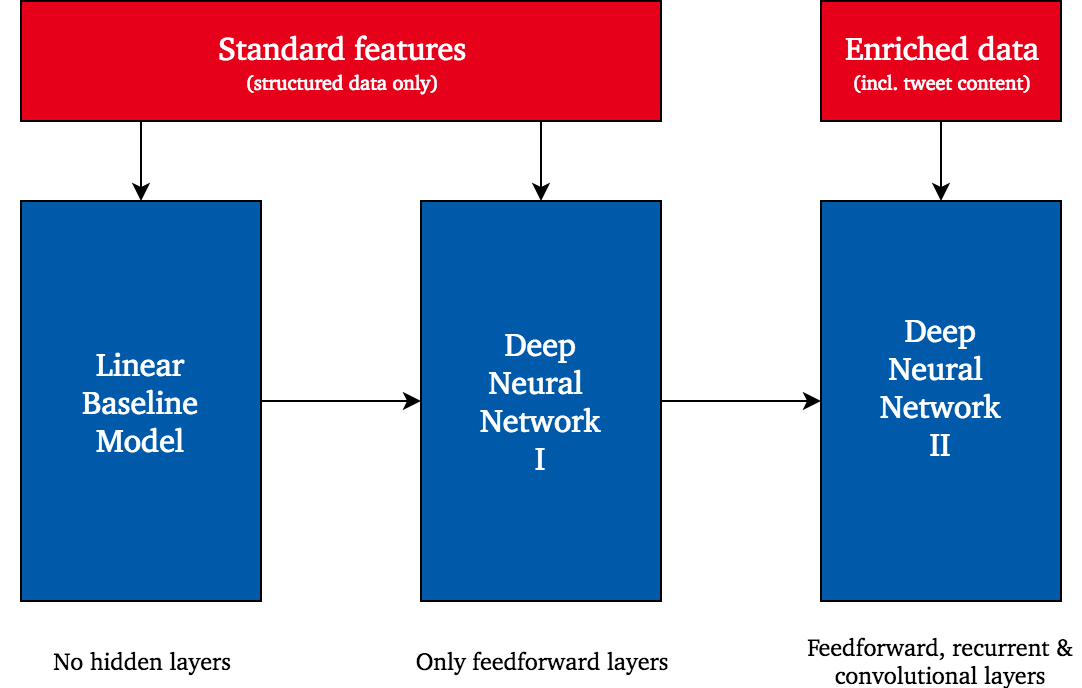
\includegraphics[height=9cm]{img/model_summary}
  \caption{Summary of developed models}
\label{fig:model_summary}
\end{figure}

Fig.~\ref{fig:model_summary} sums up the intended model evolution for this thesis.
Each model will be used in both a regression and multi-class classification
setting, producing separate predictions for retweet and favorite counts.
In order to enable comparisons, a linear baseline model will be created first.
This model will be trained solely using structured data.
In their essence, these models represent linear and logistic regression models
respectively.
Afterwards, a deep neural network is trained on the same structured data sets.
This model employs standard feed-forward layers (see ch.~\ref{sub:dl_concepts}),
which enables more complex input representations and hence more accurate
predictive outputs.
The final model is trained using enriched, i.e., structured and unstructured,
input data and more sophisticated layer architectures.
Both convolutional and recurrent layers are deployed in order to derive more
powerful features from the tweet content. 
Including textual input data requires additional preprocessing steps which aim
to transform words into floating-point numbers.
However, these additional steps do not hinder the practical applicability
of the model since they are not costly computation-wise.

\subsubsection{Assumptions}

This work relies on the assumption that most retweeting occurs in a short time
span after tweet creation.
Following this assumption, retweet and favorite counts can be approximated
to be precise estimates of the tweet engagement one month after the initial
creation.
This important assumption can be justified by research which conducts analysis
on large tweet data sets.
The overall conclusion of such research is that half of retweeting occurs within
hours, and more than 90 \% within one month after tweet publication~\footcite{Kwak2010, Kupavskii2012, Zaman2014}.

Having established intended experiments for this work, the concluding section
in this methodology chapter will describe the examined data sets and the
collection process.
